% Options for packages loaded elsewhere
\PassOptionsToPackage{unicode}{hyperref}
\PassOptionsToPackage{hyphens}{url}
%
\documentclass[
  11pt,
]{article}
\usepackage{amsmath,amssymb}
\usepackage{setspace}
\usepackage{iftex}
\ifPDFTeX
  \usepackage[T1]{fontenc}
  \usepackage[utf8]{inputenc}
  \usepackage{textcomp} % provide euro and other symbols
\else % if luatex or xetex
  \usepackage{unicode-math} % this also loads fontspec
  \defaultfontfeatures{Scale=MatchLowercase}
  \defaultfontfeatures[\rmfamily]{Ligatures=TeX,Scale=1}
\fi
\usepackage{lmodern}
\ifPDFTeX\else
  % xetex/luatex font selection
\fi
% Use upquote if available, for straight quotes in verbatim environments
\IfFileExists{upquote.sty}{\usepackage{upquote}}{}
\IfFileExists{microtype.sty}{% use microtype if available
  \usepackage[]{microtype}
  \UseMicrotypeSet[protrusion]{basicmath} % disable protrusion for tt fonts
}{}
\makeatletter
\@ifundefined{KOMAClassName}{% if non-KOMA class
  \IfFileExists{parskip.sty}{%
    \usepackage{parskip}
  }{% else
    \setlength{\parindent}{0pt}
    \setlength{\parskip}{6pt plus 2pt minus 1pt}}
}{% if KOMA class
  \KOMAoptions{parskip=half}}
\makeatother
\usepackage{xcolor}
\usepackage[margin=1in]{geometry}
\usepackage{longtable,booktabs,array}
\usepackage{calc} % for calculating minipage widths
% Correct order of tables after \paragraph or \subparagraph
\usepackage{etoolbox}
\makeatletter
\patchcmd\longtable{\par}{\if@noskipsec\mbox{}\fi\par}{}{}
\makeatother
% Allow footnotes in longtable head/foot
\IfFileExists{footnotehyper.sty}{\usepackage{footnotehyper}}{\usepackage{footnote}}
\makesavenoteenv{longtable}
\usepackage{graphicx}
\makeatletter
\def\maxwidth{\ifdim\Gin@nat@width>\linewidth\linewidth\else\Gin@nat@width\fi}
\def\maxheight{\ifdim\Gin@nat@height>\textheight\textheight\else\Gin@nat@height\fi}
\makeatother
% Scale images if necessary, so that they will not overflow the page
% margins by default, and it is still possible to overwrite the defaults
% using explicit options in \includegraphics[width, height, ...]{}
\setkeys{Gin}{width=\maxwidth,height=\maxheight,keepaspectratio}
% Set default figure placement to htbp
\makeatletter
\def\fps@figure{htbp}
\makeatother
\setlength{\emergencystretch}{3em} % prevent overfull lines
\providecommand{\tightlist}{%
  \setlength{\itemsep}{0pt}\setlength{\parskip}{0pt}}
\setcounter{secnumdepth}{5}
\newlength{\cslhangindent}
\setlength{\cslhangindent}{1.5em}
\newlength{\csllabelwidth}
\setlength{\csllabelwidth}{3em}
\newlength{\cslentryspacingunit} % times entry-spacing
\setlength{\cslentryspacingunit}{\parskip}
\newenvironment{CSLReferences}[2] % #1 hanging-ident, #2 entry spacing
 {% don't indent paragraphs
  \setlength{\parindent}{0pt}
  % turn on hanging indent if param 1 is 1
  \ifodd #1
  \let\oldpar\par
  \def\par{\hangindent=\cslhangindent\oldpar}
  \fi
  % set entry spacing
  \setlength{\parskip}{#2\cslentryspacingunit}
 }%
 {}
\usepackage{calc}
\newcommand{\CSLBlock}[1]{#1\hfill\break}
\newcommand{\CSLLeftMargin}[1]{\parbox[t]{\csllabelwidth}{#1}}
\newcommand{\CSLRightInline}[1]{\parbox[t]{\linewidth - \csllabelwidth}{#1}\break}
\newcommand{\CSLIndent}[1]{\hspace{\cslhangindent}#1}
\ifLuaTeX
\usepackage[bidi=basic]{babel}
\else
\usepackage[bidi=default]{babel}
\fi
\babelprovide[main,import]{ngerman}
% get rid of language-specific shorthands (see #6817):
\let\LanguageShortHands\languageshorthands
\def\languageshorthands#1{}
\usepackage{float}
\ifLuaTeX
  \usepackage{selnolig}  % disable illegal ligatures
\fi
\IfFileExists{bookmark.sty}{\usepackage{bookmark}}{\usepackage{hyperref}}
\IfFileExists{xurl.sty}{\usepackage{xurl}}{} % add URL line breaks if available
\urlstyle{same}
\hypersetup{
  pdftitle={Quantitative Zeitreihenanalyse der Medienberichterstattung und dem Wandel der Öffentlichen Stimmung zur Flüchtlingskrise 2015/2016},
  pdfauthor={Lasse Rodeck, Matrikel Nr.: 6906226; Seminartitel: Zur medialen und sozialen Strukturierung Politischen Konflikts und Zusammenhalts; Seminar‐Nr.: 24-108.26; Modul: Vertiefungsmodul; Dozent: Dr.~Matthias Revers},
  pdflang={de-DE},
  hidelinks,
  pdfcreator={LaTeX via pandoc}}

\title{Quantitative Zeitreihenanalyse der Medienberichterstattung und
dem Wandel der Öffentlichen Stimmung zur Flüchtlingskrise 2015/2016}
\usepackage{etoolbox}
\makeatletter
\providecommand{\subtitle}[1]{% add subtitle to \maketitle
  \apptocmd{\@title}{\par {\large #1 \par}}{}{}
}
\makeatother
\subtitle{Automatisierte Textanalyse und Medieneinfluss im Fokus}
\author{Lasse Rodeck, Matrikel Nr.: 6906226 \and Seminartitel: Zur
medialen und sozialen Strukturierung Politischen Konflikts und
Zusammenhalts \and Seminar‐Nr.: 24-108.26 \and Modul:
Vertiefungsmodul \and Dozent: Dr.~Matthias Revers}
\date{Samstag 26 August, 2023}

\begin{document}
\maketitle
\begin{abstract}
Diese Hausarbeit untersucht die Entwicklung des Sentiments in
derBerichterstattung über Flüchtlinge in Deutschland während der
Flüchtlingskrise 2015/2016. Die Analyse konzentriert sich auf die `Wir
schaffen das!'-Rede von Angela Merkel am 31. August 2015 und die
Silvesternacht 2015/2016. Mittels Sentimentanalyse und Themenclustering
werden Artikel aus den Online-Zeitungen Bild Online und Spiegel Online
verglichen. Die Ergebnisse zeigen, dass das Sentiment zu Beginn positiv
war und sich im Laufe der Zeit negativ veränderte, wobei beide Zeitungen
diese Entwicklung widerspiegelten. Die Studie bietet Einblicke in die
Rolle der Medien bei der Wahrnehmung der Flüchtlingskrise. Die
Verwendung von Natural Language AI-Modellen ermöglicht eine umfassende
Analyse großer Textmengen. Die Ergebnisse tragen zur Reflexion über den
Medieneinfluss auf die öffentliche Meinung bei und bieten eine Grundlage
für zukünftige Forschung über die Berichterstattung zu gesellschaftlich
relevanten Themen.
\end{abstract}

\renewcommand*\contentsname{Inhaltsverzeichnis}
{
\setcounter{tocdepth}{2}
\tableofcontents
}
\listoffigures
\listoftables
\setstretch{1.5}
\textbf{Eigenständigkeitserklärung}

Rodeck, Lasse 6906226 Hiermit erkläre ich, Lasse Rodeck, dass ich die
vorliegende Arbeit eigenständig, ohne fremde Hilfe und nur unter
Verwendung der angegebenen Hilfsmittel angefertigt habe. Alle sinngemäß
und wörtlich übernommenen Textstellen aus der Literatur bzw. dem
Internet habe ich als solche kenntlich gemacht. Mir ist bekannt, dass im
Falle einer Täuschung die Abschlussarbeit als „nicht bestanden''
bewertet wird.

Hamburg, Samstag 26 August, 2023


\includegraphics[width=2.19792in,height=\textheight]{images/Signature Digital.png}

\pagebreak

\hypertarget{einleitung}{%
\section{Einleitung}\label{einleitung}}

Die Flüchtlingskrise von 2015/2016 stellte Deutschland vor eine der
größten gesellschaftlichen Herausforderungen der jüngeren Geschichte. In
dieser Zeit wurden zwei besonders bedeutende Ereignisse medial intensiv
diskutiert: Angela Merkels wegweisende „Wir schaffen das"-Rede am 31.
August 2015 und die Vorfälle in der Silvesternacht 2015/2016. Die
Berichterstattung über diese Ereignisse in den Medien hatte einen
erheblichen Einfluss auf die öffentliche Meinung und die Wahrnehmung von
Flüchtlingen in Deutschland.

Diese Hausarbeit widmet sich der Analyse der Entwicklung des Sentiments
in der Berichterstattung über Flüchtlinge in Deutschland im Kontext der
oben genannten Ereignisse. Dabei liegt der Fokus auf einem Vergleich der
Artikelarchive zweier prominenter Online-Zeitungen: Bild Online und
Spiegel Online (SPON). Die Forschungsfrage dieser Hausarbeit lautet:
„\emph{Wie hat sich das Sentiment der untersuchten Veröffentlichungen im
untersuchten Zeitraum verändert?"} Ich stelle hier zu die Hypothese auf,
dass ein Abfall der Stimmung der Artikel von Sommer 2015 bis Frühjahr
2016 beobachtet werden kann. Dies würde das von Haller (2017)
beschriebene Phänomen bestätigen.

Haller (2017) analysierten bereits Ton und Inhalt des gleichen Zeitraums
und kamen zu dem Schluss, dass Leitmedien vor allem Aussagen staatlicher
und politischer Akteure als Quelle nahmen. Ihre Studie „ergab, dass in
der Kategorie der relevanten Akteure und Sprecher zwei von drei
Nennungen zur institutionellen Politik zählen'' (Ebd. S. 133). Diese
Leitmedien werden dabei unter dem Theorem der Agenda Setting betrachtet.
Da diese Hausarbeit ein ähnliches Ziel verfolgt wie Haller (2017), werde
ich mich ebenfalls auf dieses Theorem beziehen. Diese Arbeit versteht
Leitmedien dabei als Meinungsmacher und betrachtet den Verlauf des
Sentiments der Berichterstattung als relevanter Einfluss auf den
öffentlichen Diskurs.

Um das Sentiment in den Artikeln zu berechnen, wird ein Natural Language
AI Model eingesetzt. Dieses moderne Analysewerkzeug ermöglicht eine
schnelle, automatisierte Sentimentanalyse großer Textmengen. Es kann die
positiven, neutralen und negativen Tendenzen in den Texten erkennen und
somit eine quantitative Basis für die Untersuchung des Sentiments
liefern. Da sich die Flüchtlingskrise 2015 facettenreich ausdrückt, wird
zur Differenzierung der Ergebnisse eine Clusterung der Texte
vorgenommen, wodurch diese in wenige verschiedene Themen eingeteilt
werden sollen. Dadurch lassen sich Veränderungen in bestimmten Bereichen
der Berichterstattung leichter aufzeigen.

Die Verwendung dieses AI-Modells bietet mehrere Vorteile. 1) ermöglicht
es eine effiziente und schnelle Analyse einer großen Anzahl von
Artikeln, was bei manueller Analyse zeitaufwändig und unpraktisch wäre.
2) wird durch die maschinelle Verarbeitung ein reproduzierbarer Ansatz
gewährleistet, da der Einfluss menschlicher Vorurteile und
Sozialisierung minimiert werden. 3) können durch die computergestützte
Analyse auch subtile Unterschiede im Sentiment erfasst werden, die für
das Gesamtbild der medialen Berichterstattung relevant sein können.

Im weiteren Verlauf dieser Hausarbeit werden die Ergebnisse der
Sentimentanalyse diskutiert, um Einblicke in die mediale Reflexion der
Flüchtlingskrise und die Rolle der Medien bei der Gestaltung der
öffentlichen Meinung zu gewinnen. Darüber hinaus werden mögliche
Einflussfaktoren auf das Sentiment und Unterschiede in der
Berichterstattung zwischen den beiden Zeitungen beleuchtet. Ziel ist es,
ein umfassendes Bild der Sentimententwicklung in der Berichterstattung
über Flüchtlinge in Deutschland zu zeichnen und deren Bedeutung für die
Gesellschaft zu reflektieren.

\hypertarget{theorie}{%
\section{Theorie}\label{theorie}}

\hypertarget{leitmedien}{%
\subsection{Leitmedien}\label{leitmedien}}

Es bietet sich an, mit einer Definition für diesen, so viel sei
verraten, noch häufig zu nennenden Begriff anzufangen. Häufig benutzt,
und doch selten präzise definiert. Haller (2017) scheinen den Begriff
vor allem Synonym für Zeitung mit großer Auflage und überregionalem
Fokus wie Süddeutsche Zeitung, Frankfurter Allgemeine Zeitung und Die
Welt (vgl. Ebd. S. 10) zu benutzen, jedoch bleiben sie eine genaue
Definition schuldig.

Jarren und Vogel (2011) hingegen stellen uns eine Definition zur
Verfügung, die auch mit dem Verständnis anderer Beiträge wie Haller
(2017) oder Entman (2003) vereinbar ist.

\begin{quote}
\emph{``Leitmedien besitzen also vor allem dann ein grosses
Wirkungspotenzial, weil und wenn sie die Eliten in Politik, Wirtschaft
und Kultur erreichen und dadurch Entscheidungen mit weit reichenden
Konsequenzen beeinflussen können oder könnten: Was die führenden Medien
aufgreifen, wird auch zum Thema der zuständigen Eliten. Leitmedien sind
hier als Meinungsführermedien anzusehen''}

Jarren und Vogel (2011)
\end{quote}

\hypertarget{die-medien-und-die-fluxfcchtlingskrise}{%
\subsection{Die Medien und die
Flüchtlingskrise}\label{die-medien-und-die-fluxfcchtlingskrise}}

Birkner u.~a. (2020) beschreiben zu Beginn der Flüchtlingskrise 2015 ein
eher harmonisches Bild der deutschen Gesellschaft. Die Medien hätten zu
Beginn vor allem positiv über das Thema berichtet. Gleichermaßen sei
auch die generelle gesellschaftliche Stimmung positiv gewesen (Ebd. S.
52). Die BILD habe z. B. mit ihrer Aktion `Wir Helfen\textquotesingle{}
geworben und alles in allem sei der Begriff 'Willkommenskultur' viel
beworben Birkner u.~a. (2020).

Haller (2017) kommt zu dem Schluss, dass in Leitmedien häufig
ausschließlich positiv berichtet wurde und Positionen der politischen
Eliten direkt oftmals unkritisch übernommen worden seien. Zwar sei die
Stimmung generell postiv gewesen (vgl. Birkner u.~a. (2020) S.52)
allerdings habe diese unkritische Berichterstattung auch in einigen
Teilen der Öffentlichkeit zur Anschauung, „der deutsche Journalismus sei
auf Regierungslinie" (S. 53). Dieser positive Trend habe bis zum Ende
des Sommers 2015 angehalten (vgl. Haller 2017, 93).

\begin{quote}
\emph{``Im Laufe des 4. Quartals kommt nun aber auch eine völlig andere
Tonlage, Stoßrichtung und Stimme im Parteienkonzert zu Gehör: Die
Akteure der „Alternative für Deutschland'' greifen das Narrativ
Willkommenskultur auf und wenden es gegen seine Promotoren. Nachdem sie
bis zum Sommer 2015 von der Presse im Kontext der Willkommenskultur kaum
beachtet worden war, wird die AfD nun als Wortführer der
Willkommenskultur-Kritiker quasi entdeckt und -- vor allem im Anschluss
an die Silvesternacht 2015/16 -- in der Presse häufiger genannt als jede
der Regierungsparteien''}

Haller (2017) S.93
\end{quote}

Die Stimmung kippte also spätestens nach der Silvesternacht von Köln,
jedoch zeigt Haller (2017) auch, dass die Grundlage für eine negativere
Berichterstattung bereits vorher gelegt wurde. Die Silvesternacht von
Köln bezeichnet ein Ereignis, bei dem „es in der Kölner Innenstadt zu
Ausschreitungen {[}kam{]}, bei denen Asylbewerber Frauen sexuell
bedrängten" (Birkner u.~a. 2020) S. 53{]}. Spätestens danach kam es zu
einem Bruch der durchweg positiven Berichterstattung. Die Springer
Presse mit BILD und WELT seien danach einen deutlich kritischeren Kurs
gefahren. Der Großteil der Medien habe sich allerdings hinter die
Flüchtlinge gestellt und Angela Merkels Linie; zusammengefasst mit ihrem
viel zitierten Ausspruch „Wir schaffen das!" {[}vgl. Ebd. S.54{]}.

\hypertarget{agenda-setting}{%
\subsection{Agenda Setting}\label{agenda-setting}}

Die Agenda Setting Theorie, eingeführt von McCombs und Shaw (1972) ist
Theorie aus dem Bereich der Medienwissenschaften. Sie versteht
Massenmedien als die Organe, die entscheiden, welche Themen Teil des
öffentlichen Diskurses werden.

\begin{quote}
\emph{``While the mass media may have little influence on the direction
or intensity of attitudes, it is hypothesized that the mass media set
the agenda for each political campaign, influencing the salience of
attitudes toward the political issues.''}

\begin{center}\rule{0.5\linewidth}{0.5pt}\end{center}

\emph{``Während die Massenmedien nur einen geringen Einfluss auf die
Richtung oder Intensität der Einstellungen haben, wird angenommen, dass
die Massenmedien die Agenda für jede politische Kampagne festlegen und
damit die Bedeutung der Einstellungen zu politischen Themen
beeinflussen.''}

McCombs und Shaw (1972)
\end{quote}

Politik und Medien werden hier in Wechselwirkung zueinander verstanden.
Poltiker:innen wählen ihre Platform für die nächste Zeit und stellen
diese vor. Der redaktionelle Teil der Massenmedien greift diese Platform
auf, aber entscheidet am Ende selbst, welchen Inhalten man mehr Platz
einräumen möchte.

Den Massenmedien kommt damit eine wichtige Rolle des öffentlichen Lebens
zu. Nicht nur entwickelt sich der öffentliche Diskurs entlang der
gesetzten Agenda, ebenfalls wird dieser Diskurs auch die politische
Arena berühren und sie in ihrer zukünftigen Ausrichtung verändern. Einen
besonderen Fall dieses Austausches beschreibt Entman (2003) mit dem
Kaskadeneffekt. Es ist ein Fall, der beschreibt, wenn Medien für
bestimmte Agendapunkte das Framing aus homogenen Quellen direkt
übernehmen. Entman (2003) beschreibt dies im Zusammenhang des
Irakkriegs, als Massenmedien meist unkritisch das Framing der
Bush-Administration übernahmen und damit einen Krieg gegen den Irak zu
einem großen Thema innerhalb des öffentlichen Diskurses machten.

\hypertarget{methode}{%
\section{Methode}\label{methode}}

\hypertarget{sentiment-analyse}{%
\subsection{Sentiment Analyse}\label{sentiment-analyse}}

Die Sentimentanalyse ist eine Methode der Textanalyse, die darauf
abzielt, das Sentiment oder die Stimmung in einem Text zu erkennen und
zu bewerten. Mithilfe eines Natural Language AI-Modells von Wiseman,
Nydick, und Wisner (2022) wird jedem Artikel ein Sentiment Score
zwischen -1 (sehr negativ) und 1 (sehr positiv) zugeordnet. Das
AI-Modell analysiert dabei den Kontext, die verwendeten Wörter und die
Satzstruktur, um das Sentiment des Textes zu ermitteln. Ein großer
Vorteil der Sentimentanalyse mittels AI-Modells besteht in ihrer
Effizienz und Skalierbarkeit. Im Vergleich zu manuellen Methoden
ermöglicht sie die schnelle und automatisierte Analyse einer großen
Anzahl von Artikeln, wodurch umfassendere Erkenntnisse über die mediale
Wahrnehmung der Flüchtlingskrise gewonnen werden können. Zudem reduziert
die Verwendung eines AI-Modells die Anfälligkeit für menschliche
Vorurteile, da die Analyse objektiver und konsistenter erfolgt.

\hypertarget{lda}{%
\subsection{LDA}\label{lda}}

Die Methode des Themenclustering mit Latent Dirichlet Allocation (LDA)
ist ein unüberwachtes Lernverfahren zur Themenmodellierung von
Textdaten. Dabei werden ähnliche Artikel aufgrund ihrer thematischen
Übereinstimmungen in Clustern zusammengefasst. LDA identifiziert latente
Themen, die in den Artikeln verborgen sind, und ordnet jeden Artikel den
entsprechenden Clustern zu. Die Methode basiert auf einer
Wahrscheinlichkeitsverteilung, die es erlaubt, die thematischen
Beziehungen in den Artikeln zu entdecken. Ein wesentlicher Vorteil von
LDA besteht in seiner Flexibilität und Fähigkeit, neue und unerwartete
Themen zu entdecken, ohne vorher definierte Kategorien zu benötigen.
Dadurch kann LDA einen tieferen Einblick in die in den Artikeln
behandelten Themen geben, die möglicherweise bei vorherigen manuellen
Kategorisierungsansätzen unentdeckt geblieben wären. Zudem ermöglicht
die Themenclustering-Analyse eine umfassendere und differenziertere
Analyse der Berichterstattung über die Flüchtlingskrise, indem sie
Artikel mit ähnlichen Schwerpunkten und Inhalten in thematischen
Clustern zusammenfasst.

\hypertarget{webscraping}{%
\subsubsection{\texorpdfstring{\textbf{Webscraping}}{Webscraping}}\label{webscraping}}

Die Datenerhebung für diese Hausarbeit erfolgte mittels Webscraping,
einer automatisierten Technik zur Extraktion von Daten von Websites.
Ziel war es, Artikel aus den Archiven zweier Online-Zeitungen, nämlich
Bild Online und SPON, zu sammeln, um eine umfangreiche Datengrundlage
für die Analyse der Entwicklung des Sentiments in der Berichterstattung
über Flüchtlinge in Deutschland 2015/2016 zu schaffen.

Das Webscraping bietet den Vorteil, eine große Menge an relevanten
Artikeln aus den Archiven der Online-Zeitungen zu extrahieren, ohne dass
dies manuell erfolgen muss. Es ermöglichte eine automatisierte
Datenerhebung, wodurch Zeit und Aufwand eingespart werden können. Die
gesammelten Artikel bilden eine unrepräsentative Stichprobe der medialen
Berichterstattung über Flüchtlinge während der untersuchten Zeiträume,
die als Basis für die weitere Analyse mittels Sentimentanalyse und
Themenclustering dienten.

\hypertarget{auswahl-der-zeitungen}{%
\subsection{Auswahl der Zeitungen}\label{auswahl-der-zeitungen}}

Diese Arbeit versucht, einen Vergleich anzubieten. Da ich vor allem an
sichtbarer Veränderung interessiert bin, ergibt es Sinn, mindestens eine
Zetung in das Datenset mit aufzunehmen, die einen besonders starken
Rechtsruck anzeigen würde. Da es häufig schwierig sein kann, die
tatsächliche editoriale Linie einer Zeitschrift zu definieren, beziehe
ich mich bei dieser Einordnung auf die angenommene politische
Ausrichtung der Leserschaft in Person der deutschen
Bundestagsabgeordneten. Barthels u.~a. (2021) zeigt, dass Bild.de vor
allem von rechtsgerichteten Parteien wie der AFD, CDU und FDP aufgerufen
werde. SPON hingegen vor allem von Abgeordneten der Grünen, SPD und
Linken. Allerdings werde der SPON auch von allen Parteien auf einem
relativ hohen Niveau genutzt.

Aus den Nutzungsstatistiken leite ich ab, dass der SPON als
Nachrichtenorgan vor allem neutral angesehen wird und daher eine gute
Basislinie für einen Vergleich zur eher rechtpopulistischen Linie der
Bild darstellen soll.

\hypertarget{ergebnisse}{%
\section{Ergebnisse}\label{ergebnisse}}

Die meisten Beobachtungen stammen aus den Feldern Politik/Ausland sowie
Panorama. Durchschnittlich gibt es 3,5 Beobachtungen pro Tag mit einer
Spannweite von 19, wobei der maximale Wert 19 Beobachtungen pro Tag
beträgt.

Mit Anfang des Septembers 2015 lässt sich ein erhöhtes Aufkommen an
Artikeln erkennen, welches seinen Hochpunkt zwischen November und
Dezember 2015 erreicht. Ursprünglich wurden alle Artikel, die verfügbar
waren und aus Text bestanden (Bildstrecken oder Videos wurden nicht
gescraped) gesammelt. Dieses Datenset wurde dann mit einem
Stichwortfilter eingegrenzt. Nach diesen Stichwörtern wurde im Titel
oder Text gesucht.

\begin{longtable}[]{@{}lr@{}}
\caption{Schlagwörter zur Suche nach relevanten Artikeln}\tabularnewline
\toprule\noalign{}
Schlagwort & Vorkommen \\
\midrule\noalign{}
\endfirsthead
\toprule\noalign{}
Schlagwort & Vorkommen \\
\midrule\noalign{}
\endhead
\bottomrule\noalign{}
\endlastfoot
Abschiebung & 74 \\
Asyl & 488 \\
Ausland & 141 \\
Ausländer & 281 \\
Flüchtling & 950 \\
Integration & 123 \\
Migranten & 300 \\
Migration & 236 \\
Nordafrika & 54 \\
Schleuser & 66 \\
Terror & 1004 \\
\end{longtable}

Diese Liste ist ohne Zweifel nicht vollständig, jedoch geht eine
genauere Methodik über den Rahmen dieser Arbeit hinaus, wäre aber für
zukünftige Arbeiten denkbar.

\hypertarget{sentiment-analyse-1}{%
\subsection{Sentiment Analyse}\label{sentiment-analyse-1}}

Ausgehend von der Birkner u.~a. (2020) ausgeführten Zeitreihe definiere
ich meinen Untersuchungszeitraum um diese zwei Events herum. Er beginnt
Juli 2015 und endet im März 2016. Es umfasst damit die beiden relevanten
Ereignisse, den `Wir schaffen das!'-Auspruch von Angela Merkel Ende
August 2015 und die Sylvesternacht in Köln mit genug Nachlauf, um
Trendveränderungen erkennen zu können.

Eine einfache Zeitreihe lässt einen negativen Trend erkennen. Der Sommer
2015 beginnt relativ positiv. Diese Einstellung nimmt jedoch bis April
2016 ab. Die Bildzeitung macht dabei einen deutlich stärkeren Wandel
durch. SPON, wenn auch mit einem leicht negativen Trend verändert sich
in Sentiment kaum. Teilweise wird hier Haller (2017) bestätigt. Beide
Zeitungen erleben eine wahrnehmbare negative Veränderung. Begann der
Trend für die Bildzeitung im beobachteten Zeitraum bei etwas über 0,15,
findet er sich am Ende bei etwas unter 0,1. Über alle Themen hinweg hat
das durchschnittliche Sentiment damit um über 5\% abgenommen.

\begin{figure}[H]
\includegraphics[width=0.7\linewidth,]{Hausarbeit_files/figure-latex/sentiment_timeseries-1} \caption{Zeitreihe Durchschnittliches Sentiment Pro Tag}\label{fig:sentiment_timeseries}
\end{figure}

In dieser Zeitreihe finden sich allerdings viele Texte, die in
irgendeiner Form Flüchtlinge erwähnen, wieder. Wie oben erwähnt wurden
nur Schlagwortsuchen benutzt, um die Artikelmenge einzugrenzen.
Tatsächlich ist allerdings anzunehmen, dass das zu beobachtende Phänomen
sich in vielen Facetten und Themen widerspiegeln wird. In dem
vorhandenen Datenset und der oben abgebildeten Zeitreihe finden sich all
diese Themen unberücksichtigt wieder. Diese könnten das durchschnittlich
gemessene Sentiment durchaus beeinflussen. Im nächsten Abschnitt soll
sich daher mit dieser Problematik befasst werden.

\hypertarget{topic-modelling-lda}{%
\subsection{Topic Modelling (LDA)}\label{topic-modelling-lda}}

Zur tieferen Betrachtung der Sentimentanalyse werden die Texte mittels
LDA-Modelling in Themen eingeteilt. Dies geschieht mittels einer
unbeaufsichtigten Lernmethode. Zur Auswahl der Menge an Clustern wurden
und Koherenz als entscheidende Faktoren für Interpretierbarkeit
herangezogen. Ich habe mich am Ende für 4 Cluster entschieden.

\begin{figure}[H]
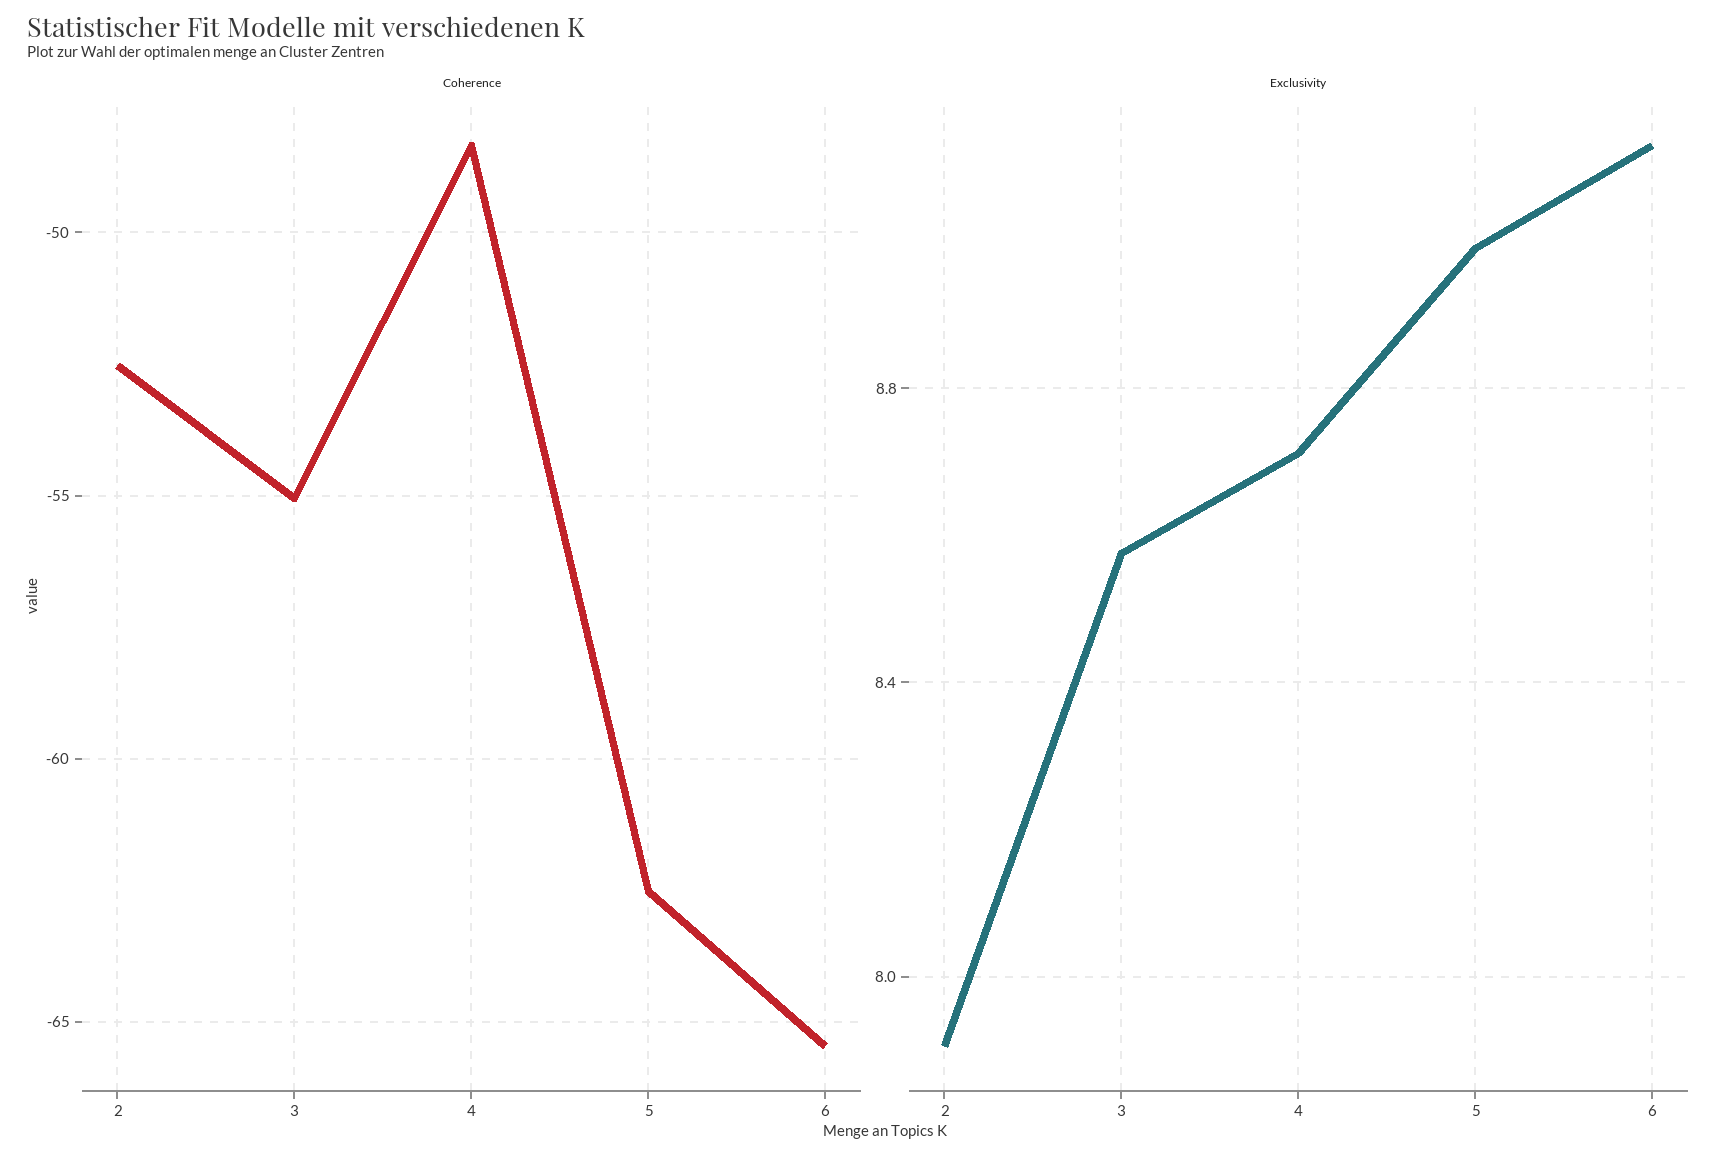
\includegraphics[width=0.5\linewidth,]{Hausarbeit_files/figure-latex/topic_model_k_selection, figures-side-1} 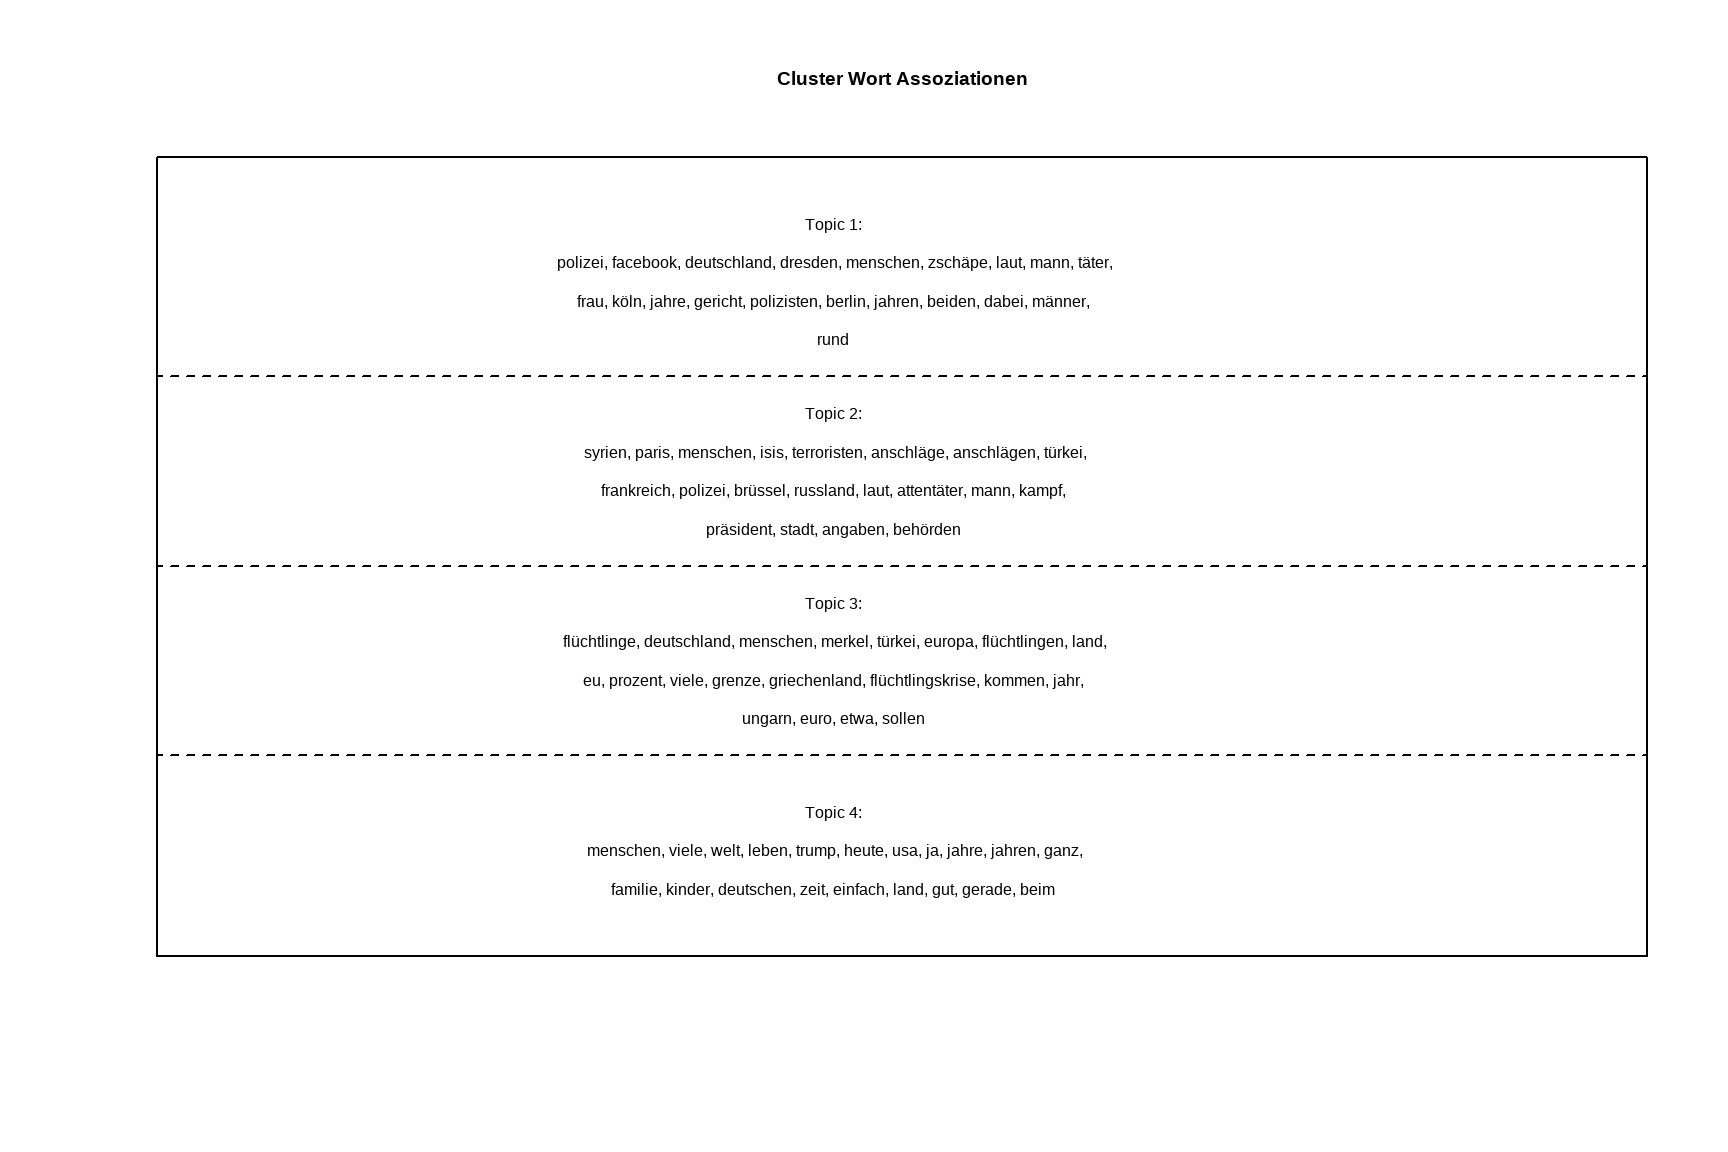
\includegraphics[width=0.5\linewidth,]{Hausarbeit_files/figure-latex/topic_model_k_selection, figures-side-2} \caption{K Means Cluster Optimum}\label{fig:topic_model_k_selection, figures-side}
\end{figure}

Von den 4 Clustern sind zumindest 3 gut interpretierbar. Auf Grundlage
der genannten hoch korrelierten Wörter habe ich die 4 Themen
`Rechtsextremismus', `Islamischer Terrorismus', `Europäische
Flüchtlingskrise' und `US-Wahl' benannt.

\hypertarget{sentimentanalyse-mit-topic-modelling-lda}{%
\subsection{Sentimentanalyse mit Topic Modelling
(LDA)}\label{sentimentanalyse-mit-topic-modelling-lda}}

Mittels der Clusterergebnisse lassen sich nun die Sentimente aufgeteilt
nach Thema ploten und ihre individuelle Entwicklung beobachten.
Tatsächlich lässt sich erkennen, dass vor allem im Thema `Europäische
Flüchtlingskrise' das Sentiment im beobachteten Zeitraum extrem gesunken
ist. Diese Beobachtung gilt für beide beobachteten Medien. Die anderen
Themen sind von dieser Entwicklung weitestgehend unbetroffen. Zwar gibt
es auch im Bereich des islamistischen Terrors eine negative Entwicklung,
jedoch nur auf Seiten der Bildzeitung\footnote{Der Spike am Ende des
  Jahres in Abbildung 3 kommt bei der Bildzeitung dadurch zu Stande,
  dass es nur einen Artikel mit einem Sentiment von 0,441 gibt; Ein
  Interview mit Entwicklungsminister Müller. Spiegel Online
  veröffentlicht in der gleichen Woche einen Artikel namens
  „Flüchtlinge: Küstenwache rettet zu Weihnachten Tausende im
  Mittelmeer'' (Score 0,486), „Silvester: An Flüchtlingsheimen in NRW
  herrscht Böller-Verbot'' (0.288), sowie „Zuwanderung: Flüchtlinge
  können für Wirtschaftswunder sorgen'' (0,155), die zu diesem Peak
  führen. Es gab nur einen Artikel, der leicht negativ war (-0,145). Es
  scheint zwischen diesen Peaks jedoch keinen Zusammenhang zu geben.}.

\begin{figure}[H]
\includegraphics[width=1\linewidth,]{Hausarbeit_files/figure-latex/sentiments_topics-1} \caption{Zeitreihe Sentiment nach Themen}\label{fig:sentiments_topics}
\end{figure}

\hypertarget{fazit}{%
\section{Fazit}\label{fazit}}

Diese Hausarbeit hat es sich zum Ziel gemacht, vor dem Hintergrund der
Flüchtlingskrise von 2015 bis 2016 mittels eines Natural Language Models
die Sentimententwicklung von Artikeln der beiden Onlineausgaben der
Leitmedien SPON und Bild zu untersuchen. Dies sollte dem Zweck dienen,
Erkenntnisse von z.B. Haller (2017) mit anderen Methoden zu überprüfen.
Mittels Topic Modelling wurden die Texte in die 4 überordnenden Themen
`Rechtsextremismus', `Islamischer Terrorismus', `Europäische
Flüchtlingskrise' und `US-Wahl' eingeteilt. Dabei lässt sich erkennen,
dass der generelle Trend vom Sommer 2015 bis Frühjahr 2016 merklich
gesunken ist. Der Beobachtungszeitraum beginnt im Sommer 2015 mit einer
leicht positiven Tendenz, nimmt im Verlauf des Jahres aber weiterhin ab
und ist am Ende des Zeitraums in das leicht negative gekippt.
Überraschend ist, dass sich dieser Trend in beiden Publikationen nahezu
identisch wiederfindet.

Diese Ergebnisse sind stimmig mit anderer Forschung wie etwa Haller
(2017). Diese fanden ebenfalls für den Anfangszeitraum eine vor allem
positive Stimmung vor und heben dabei besonders das Narrativ der
`Willkommens Kultur' hervor (Ebd. S. 99). Ebenso beschreiben sie, dass
während der Berichterstattung häufig die Positionen der politischen
Eliten wiedergegeben wurden und diese dadurch dem Theorem der Agenda
Setting folgend besonders viel Platz im öffentlichen Diskurs eingeräumt
bekamen (Ebd. S. 134). Nachdem wir gezeigt haben, dass das sich
wandelnde Sentiment tatsächlich reproduzierbar zu zeigen ist, könnte
dies ein erster Schritt sein, eine Beobachtung wie der von Entman (2003)
beschriebene Kaskadeneffekt nachzuweisen. Haller (2017) beobachtungen
bezüglich der bezogenen Quellen der Leitmedien geben ebenfalls bereits
starke Hinweise auf diese Vermutung.

Daraus lässt sich eine interessante These ableiten, die es in den
folgenden Studien zu überprüfen gilt. Wie Haller (2017) beschreibt,
waren die von Entman (2003) beschriebenen Kaskadeneffekte über den
gesamten Zeitraum zu beobachten. Allerdings haben sich die politischen
Orientierungen der befragten politischen Eliten von den
Regierungsparteien überproportional zur AfD verändert. In diesem
Zusammenhang muss die Frage erlaubt sein, ob der Stimmungsumschwung
gegenüber den nach Deutschland kommenden Flüchtlingen nicht vor allem
durch die Medien beeinflusst wurde und damit das Erstarken rechter
Parteien in Deutschland.

Weiterhin zeigt diese Arbeit, dass automatisierte Textverarbeitung
schnelle und effiziente Studien mit tausenden Textdokumenten als
Datengrundlage deutlich vereinfacht. Gerade unter dem Thema Open Data
kann dies ein entscheidender Fortschritt in der Sozial- und
Medienwissenschaftlichen Forschung sein. Mit Blick auf die Zukunft wäre
es allerdings wünschenswert, spezifischere Modelle zur Verfügung zu
haben, deren Trainingssets öffentlich einsehbar sind. Denn obwohl die
Berechnungen des AI-Modells durchaus schlüssig sind, ist es am Ende
unmöglich zu interpretieren, warum das Model zu dem Schluss kam, zu dem
es gegkommen ist. Zudem sollten generelle Standards im Umgang mit schwer
interpretierbaren Machine-Learning Modellen gefördert und genauso
gelehrt werden. An dieser Stelle muss von Forschungsseite dringend
nachgebessert werden.

Weiterführende Arbeiten könnten sich mit der Analyse der Akteure
innerhalb der Artikel, die in diesem Datenset gesammelt wurden,
beschäftigen, um die Erkenntnisse von Haller (2017), dass die meisten
Quellen oftmals aus politischen Eliten stammen, zu überprüfen. Auch dies
sollte mit Machine-Learning-Modellen effizient zu gestalten sein.

\hypertarget{packagenutzung}{%
\section*{Packagenutzung}\label{packagenutzung}}

Für Datentransformation und das Erstellen von Plots wurde das
Tidyverse-Package (Wickham u.~a. 2019) )benutzt. Webscraping wurde mit
hilfe des Rvest Packages durchgeführt (Wickham 2022). Sentimentanalysen
wurden mit Sentiment.ai (Wiseman, Nydick, und Wisner 2022) durchgeführt.
Topic Modelling wurde mit den Libraries von Benoit u.~a. (2018),
Roberts, Stewart, und Tingley (2019) und Grün und Hornik (2023)
erstellt. Tabellen wurden mit Huntington-Klein (2023) erstellt. Da das
Scrapen und Auswerten mittels AI Model sehr lange dauert, möchte ich
auch besonders Csárdi und FitzJohn (2019) erwähnen, welche mir das Leben
stark durch einen einfachen Progress Bar sehr vereinfacht haben.

\hypertarget{anmerkung}{%
\subsection*{Anmerkung}\label{anmerkung}}

Code und Datensets finden sich unter
\url{https://github.com/lrodeck/Hausarbeit-MedSoz-Stru-Pol-Kon-Zus}

\hypertarget{literatur--und-packageverzeichnis}{%
\section*{Literatur- und
Packageverzeichnis}\label{literatur--und-packageverzeichnis}}

\hypertarget{refs}{}
\begin{CSLReferences}{1}{0}
\leavevmode\vadjust pre{\hypertarget{ref-Barthels2021Die}{}}%
Barthels, Inga, Benedikt Brandhofer, Jesse Lehrke, Helena Wittlich, Finn
Müller-Hansen, und Hendrik Lehmann. 2021. {„Die {Lieblingsmedien} der
{Parteien} im {Bundestag}``}.
https://interaktiv.tagesspiegel.de/lab/die-lieblingsmedien-der-parteien/.

\leavevmode\vadjust pre{\hypertarget{ref-quanteda}{}}%
Benoit, Kenneth, Kohei Watanabe, Haiyan Wang, Paul Nulty, Adam Obeng,
Stefan Müller, und Akitaka Matsuo. 2018. {„quanteda: An R package for
the quantitative analysis of textual data``} 3: 774.
\url{https://doi.org/10.21105/joss.00774}.

\leavevmode\vadjust pre{\hypertarget{ref-Birkner2020Der}{}}%
Birkner, Thomas, Daniel König, Sebastian Mallek, Niklas Näsemann, und
Kirsten Specking. 2020. {„Der {Fall} {Angela} {Merkel} und die
'{Fl}{ü}chtlingskrise' seit 2015``}. In \emph{Krisenkommunikation
komplex: 11 {Analysen} prominenter {F}{ä}lle mit medialer {Einordnung}
und {Nachbetrachtung} beteiligter {Experten}}, herausgegeben von Jana
Wiske. K{ö}ln: Herbert von Halem Verlag.

\leavevmode\vadjust pre{\hypertarget{ref-progress}{}}%
Csárdi, Gábor, und Rich FitzJohn. 2019. {„progress: Terminal Progress
Bars``}. \url{https://CRAN.R-project.org/package=progress}.

\leavevmode\vadjust pre{\hypertarget{ref-entman2003}{}}%
Entman, Robert M. 2003. {„Cascading Activation: Contesting the White
House's Frame After 9/11``}. \emph{Political Communication} 20 (4):
415--32. \url{https://doi.org/10.1080/10584600390244176}.

\leavevmode\vadjust pre{\hypertarget{ref-topicmodels}{}}%
Grün, Bettina, und Kurt Hornik. 2023. {„topicmodels: Topic Models``}.
\url{https://CRAN.R-project.org/package=topicmodels}.

\leavevmode\vadjust pre{\hypertarget{ref-haller2017fluchtlingskrise}{}}%
Haller, Michael. 2017. {„Die „Fl{ü}chtlingskrise ``in den Medien``}.
\emph{The refugee crisis in the media{]}, OBS-Arbeitsheft} 93.

\leavevmode\vadjust pre{\hypertarget{ref-vtable}{}}%
Huntington-Klein, Nick. 2023. {„vtable: Variable Table for Variable
Documentation``}. \url{https://CRAN.R-project.org/package=vtable}.

\leavevmode\vadjust pre{\hypertarget{ref-jarren2011}{}}%
Jarren, Otfried, und Martina Vogel. 2011{„{,,}Leitmedien{``} als
Qualitätsmedien. Theoretisches Konzept und Indikatoren``}. In, 17--29.
VS Verlag für Sozialwissenschaften.
\url{https://doi.org/10.1007/978-3-531-93084-8_2}.

\leavevmode\vadjust pre{\hypertarget{ref-mccombs1972agenda}{}}%
McCombs, Maxwell E, und Donald L Shaw. 1972. {„The agenda-setting
function of mass media``}. \emph{Public opinion quarterly} 36 (2):
176--87.

\leavevmode\vadjust pre{\hypertarget{ref-stm}{}}%
Roberts, Margaret E., Brandon M. Stewart, und Dustin Tingley. 2019.
{„{\textbraceleft}stm{\textbraceright}: An
{\textbraceleft}R{\textbraceright} Package for Structural Topic
Models``} 91. \url{https://doi.org/10.18637/jss.v091.i02}.

\leavevmode\vadjust pre{\hypertarget{ref-rvest}{}}%
Wickham, Hadley. 2022. {„rvest: Easily Harvest (Scrape) Web Pages``}.
\url{https://CRAN.R-project.org/package=rvest}.

\leavevmode\vadjust pre{\hypertarget{ref-tidyverse}{}}%
Wickham, Hadley, Mara Averick, Jennifer Bryan, Winston Chang, Lucy
D'Agostino McGowan, Romain François, Garrett Grolemund, u.~a. 2019.
{„Welcome to the {\textbraceleft}tidyverse{\textbraceright}``} 4: 1686.
\url{https://doi.org/10.21105/joss.01686}.

\leavevmode\vadjust pre{\hypertarget{ref-sentiment.ai}{}}%
Wiseman, Ben, Steven Nydick, und Tristan Wisner. 2022. {„sentiment.ai:
Simple Sentiment Analysis Using Deep Learning``}.
\url{https://CRAN.R-project.org/package=sentiment.ai}.

\end{CSLReferences}

\end{document}
